\documentclass[tikz]{standalone}
\usepackage{amsmath,mathtools}
\usetikzlibrary{positioning,calc}
\begin{document}
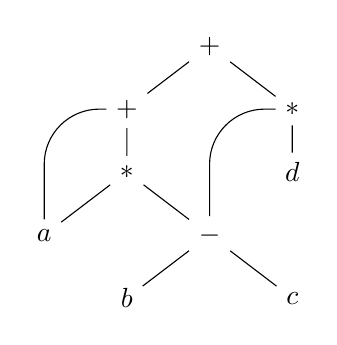
\begin{tikzpicture}[
  level distance = 8mm,
  sibling distance = 21mm,
  ]
  \node{\(+\)}
  child {
    node (p1) {\(+\)}
    child {
      node{\(*\)}
      child {
        node (s1) {\(a\)}
      }
      child {
        node (s2) {\(-\)}
        child {
          node{\(b\)}
        }
        child {
          node{\(c\)}
        }
      }
    }
  }
  child {
    node (p2) {\(*\)}
    child {
      node{\(d\)}
    }
  };

  \path[rounded corners=7mm,draw]
  (p1) -| (s1)
  (p2) -| (s2);
\end{tikzpicture}
\end{document}
